% --------------------------------------------------------------
% This is all preamble stuff that you don't have to worry about.
% Head down to where it says "Start here"
% --------------------------------------------------------------

\documentclass[11pt]{article}

\usepackage{geometry}
\usepackage{amsmath,amsthm,amssymb,url}
\usepackage{fullpage}
\usepackage{tabularx}
\usepackage{float}

\usepackage{graphicx}
\usepackage{xcolor}
\definecolor{darkblue}{rgb}{0,0,0.5} 
\usepackage{transparent}

%\addtolength{\topmargin}{-.5in}
%\addtolength{\textheight}{1.2in}

\newcommand{\N}{\mathbb{N}}
\newcommand{\Z}{\mathbb{Z}}

\newenvironment{theorem}[2][Theorem]{\begin{trivlist}
\item[\hskip \labelsep {\bfseries #1}\hskip \labelsep {\bfseries #2.}]}{\end{trivlist}}
\newenvironment{lemma}[2][Lemma]{\begin{trivlist}
\item[\hskip \labelsep {\bfseries #1}\hskip \labelsep {\bfseries #2.}]}{\end{trivlist}}
\newenvironment{exercise}[2][Exercise]{\begin{trivlist}
\item[\hskip \labelsep {\bfseries #1}\hskip \labelsep {\bfseries #2.}]}{\end{trivlist}}
\newenvironment{problem}[2][Problem]{\begin{trivlist}
\item[\hskip \labelsep {\bfseries #1}\hskip \labelsep {\bfseries #2.}]}{\end{trivlist}}
\newenvironment{question}[2][Question]{\begin{trivlist}
\item[\hskip \labelsep {\bfseries #1}\hskip \labelsep {\bfseries #2.}]}{\end{trivlist}}
\newenvironment{corollary}[2][Corollary]{\begin{trivlist}
\item[\hskip \labelsep {\bfseries #1}\hskip \labelsep {\bfseries #2.}]}{\end{trivlist}}

\begin{document}

% --------------------------------------------------------------
%                         Start here
% --------------------------------------------------------------

\title{Project outline \--- Distributed Systems}
\author{Shumo Chu and Dominik Moritz}
\date{}

\maketitle

\section{Background}

Database system need to transform user's high level queries, eg. SQL, Datalog into physical query plan for the execution. Physical query plan is the actual execution map of a database system. Usually it can be viewed as a \emph{DAG} which consists of basic operators, such as \emph{JOIN}, \emph{GROUP BY}, \emph{SCAN}, \emph{APPLY} and relational tables. In distributed database systems, the introduction of the \emph{SHUFFLE} operator and data partitioning makes query plans more complicated. All operators are distributed over a number of nodes.

Myria is a distributed big data management system currently being developed in the database group. Myria aims towards building a distributed database platform to provide \emph{big data management and analytics as a service} for scientific and many other applications.

\section{Objective}

We propose a project that will help us to understand the execution of physical query plans in the Myria database. It will allow us to efficiently debug and improve query execution.

We will develop a system that will allow us to collect information about the execution of a physical query plan in the distributed system. The data has to be collected on one node and then aggregated to provide the foundation for analyzing the data and creating a meaningful visualization. We also plan to analyze the query execution and find problems such as data skew. The visualization will be embedded in a web application. We plan to use a gantt chart to visualize events happening in operators over time. The visualization will also show the relationships between operators and their location.

\vspace{10px}

\noindent Questions that we want to answer in this project:

\begin{enumerate}
	\item What are the data dependencies between operators in workers?
	\item What is the bottleneck of the execution? Improving which part could best boost the performance?
		%\item How does an optimization rule affect query execution?
	%\item Is an execution network or CPU bound?
	\item How does network and computation contribute to the total running time? We make two hypothesis, respectively. If we assume the network has infinite bandwidth and no latency, how would the running time change. If we assume that we have infinite computation power, how would the running time change.
	\item Is there a slow worker during a certain stage of the execution that prevent the progress of the whole query plan?
	%\item How good is the load balancing? If it is skewed, how much does this affect the performance?

\end{enumerate}

Visualizing the physical execution will allows us to understand, debug and eventually improve how queries are executed.

\section{Methodoloy}
\subsection{Problem formulation}
\label{sec:formulation}

Database system profiling has been extensively studied over decades. There are two types of works on this topic. One is logging query execution information and analyzing logs afterwards for better query optimization. The other is using real-time profiling information to estimate the progress of a query. We focus on the first type of problem in the context of distributed database system.

\begin{figure}
 \begin{center}
     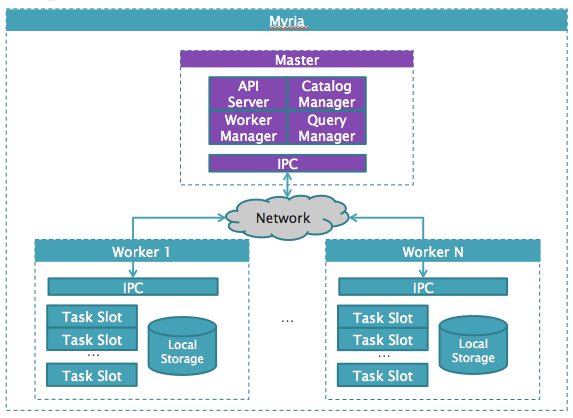
\includegraphics[width=0.7\textwidth]{myria.png}
   \end{center}
  \caption{distributed database architecture}
  \label{fig:myria_arc}
\end{figure}


\noindent\textbf{Distributed database system.} is a database system deployed on a cluster of servers.  Figure \ref{fig:myria_arc} shows the system architecture of the distributed database system we use. There is a master server who parses the query and distribute the tasks the each computing node (worker). The data is also pre-partitioned and stored in each work.  The database query in the form of SQL or Datalog will be translated to the physical query plan and then be executed.

\noindent\textbf{Query Plan.} Query plan is the actually execution map for the distributed database system.  Each query plan is consisted by basic operators forming a execution flow.   For example,   the SQL query $SELECT \; R.*, S.*  \; WHERE \; R.x=S.y ;$ can be translated to the visualized query plan showed in Figure \ref{fig:query_plan}.  The semantic of the query plan is a distributed hash join of two tables, $R$ and $S$. We need to first hash each table according to the joined fields. Then shuffle tuples by their hash results to different workers. At each worker, join the shuffled tuples locally. 


\begin{figure}
 \begin{center}
     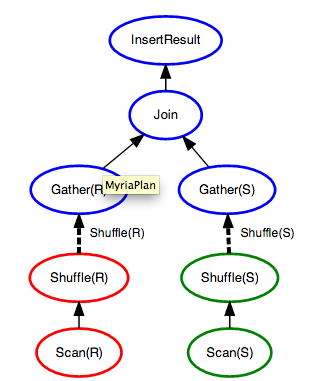
\includegraphics[width=0.4\textwidth]{partition_join.png}
   \end{center}
  \caption{query plan: distributed hash join}
  \label{fig:query_plan}
\end{figure}


% explain what we want to learn about operators, query fragments and workers
% talk about shared memory model

\subsection{Proposed implementation}
	\subsubsection*{Logging}

	As described in Section~\ref{sec:formulation}, we want to capture the state of operators, query fragments, and workers. The state of a query fragment depends on the state of the operators inside it and the state of a worker depends on the state of the query fragments that are running on it. Consequently, we only need to capture the state of query fragments per worker. In order to capture state changes, we log events and state changes of operators. In the logs we look for events that indicate a state change and signals. We use the term \emph{state} to describe the state of an operator and the term \emph{signal} to describe important events that happen at a certain point in time. For each state we want to visualize when the transitions happened.

	Not all operators have the same states. A consumer for example does not have a wait, compute or send state. Table~\ref{tbl:state} shows the different states operators can be in and briefly describes their meaning.

\begin{table}[h]
\begin{tabularx}{\textwidth}{ l|X|X|X }
 & \multicolumn{3}{ c }{operator type} \\
\cline{2-4}
state & producers & consumers & operations \newline (\emph{JOIN}, \emph{MERGE}, \emph{SCAN}, \emph{APPLY}, ...) \\
\hline \hline
receive & - & receiving data from producer over network & - \\
\hline
wait & child is producing & - & waiting for child to return \\
\hline
compute & hashing data & - & in \texttt{fetchNextReady} and not waiting for any data \\
\hline
sleep & has data for consumer that is not ready & no data in producer & waiting for signal \\
\hline
send & sending data to consumer over network & - & - \\
\end{tabularx}
\caption{Possible states of operators and their meaning.}
\label{tbl:state}
\end{table}

In order to capture these states we have to log events that indicate their beginning and their end. An operator can only be in one state at a time. Consequently, the states can be reconstructed from the logs without any information about which events belong to each other. Since we also log the time of the events we can reconstruct when an operator changes its state and determine how long it has been in a certain state.

No all transitions between states are possible. For example, the wait state can only be reached from the compute state. A way to interpret this is that wait and compute are a sub-states of another state work. This is shown in Figure~\ref{fig:extd_compute}. This interpretation is useful since a set of computes and waits can be grouped together because they were triggered by a call to \texttt{fetchNextReady} and end with a return from the function. We will use this information in the visualization of operator states.

\begin{figure}[h]
  \begin{center}
    \def\svgwidth{0.35\columnwidth}
    \input{wait_states.pdf_tex}
  \end{center}
  \caption{Extended automaton for alternative interpretation where the wait state and the compute state are sub states of a work state.}
  \label{fig:extd_compute}
\end{figure}

To be able to reconstruct the states mentioned in Table~\ref{tbl:state} we have to log all events that cause state changes. Furthermore, we will log signals. % todo: do we actually need signals?

As mentioned in the beginning of this section, the states of query fragments and workers can be inferred from the state of the query fragments that are executed on a worker. A query fragment can be in the state receiving when the leave operator is a consumer (and not a scan). It can be in the state compute when any of its children are computing. It can be sleeping when the root is sleeping and it can be sending when the root is sending. Since a fragment is executed by one thread, it cannot be in multiple states.

The state of a worker is ambiguous because multiple threads can be executing multiple query fragments that are in different states. We will use the state of the query fragments to show how many query fragments are working but we will not determine a single state for the whole worker.

% state changes

For logging, we use standard Java logging using \emph{slf4j}\footnote{\url{http://www.slf4j.org/}}, a logging API which is implemented by different logging frameworks. Since logs are collected on different workers, we need to collect them on one machine that analyzes the data and creates the visualizations. We plan to use \emph{Apache Flume}\footnote{\url{https://flume.apache.org/}} to collect the logs from the workers. Since the collecting server is a Myria worker, we can use its database to store the logs and then read from when we create the visualization. In order to do that, we will have to implement a custom Flume sink.

% how does the visualization server process the data

	\subsubsection*{Visualization}
	% Web client
	% Form of visualization, e.g. what do we visualize, operator, query fragment, workers. In each kind of visualization, how will the interface looks like.
	% What kind of information a potential user can get from the visualization.

	We will use a gantt chart to visualize the states and the times an operator or query fragment is in a state. Gantt charts are used widely in the visualization of project plans because they visualize time spans and show dependencies between them. For the visualization of operators we want to show the hierarchical relationship between operators and allow users to focus only on certain operators.

\begin{figure}[h]
  \begin{center}
    \def\svgwidth{0.9\columnwidth}
    \input{gantt.pdf_tex}
  \end{center}
  \caption{A prototype gantt chart. Red is computing, blue is waiting, gray is sleeping, and yellow is receiving.}
  \label{fig:gantt}
\end{figure}

	\emph{d3}\footnote{\url{http://d3js.org/}} will be used to build the custom visualization. D3 is a JavaScript framework for data visualizations on the web. Consequently, our visualization will be browser based and we plan to integrate it in the existing web interface for myria\footnote{a demo can be found at \url{http://myria-web.appspot.com/}}. Figure~\ref{fig:gantt} shows a mock-up of what the visualization of operators in a query fragment will look like. 

	%\subsubsection*{Analytics}
	\subsubsection*{Estimate computation/network overhead}

%\section{Result}
%\section{Summary}


\end{document}